%%%%%%%%%%%%%%%%%%%%%%%%%%%%%%%%%%%%%%%%%
% Simple Sectioned Essay Template
% LaTeX Template
%
% This template has been downloaded from:
% http://www.latextemplates.com
%
% Note:
% The \lipsum[#] commands throughout this template generate dummy text
% to fill the template out. These commands should all be removed when
% writing essay content.
%
%%%%%%%%%%%%%%%%%%%%%%%%%%%%%%%%%%%%%%%%%

%----------------------------------------------------------------------------------------
%	PACKAGES AND OTHER DOCUMENT CONFIGURATIONS
%----------------------------------------------------------------------------------------

\documentclass[12pt]{article} % Default font size is 12pt, it can be changed here

\usepackage{geometry} % Required to change the page size to A4
\geometry{a4paper} % Set the page size to be A4 as opposed to the default US Letter

\usepackage{graphicx} % Required for including pictures

\usepackage{float} % Allows putting an [H] in \begin{figure} to specify the exact location of the figure
\usepackage{wrapfig} % Allows in-line images such as the example fish picture

\usepackage{lipsum} % Used for inserting dummy 'Lorem ipsum' text into the template

\usepackage{multicol}
\usepackage{amsmath}

\usepackage[utf8x]{inputenc}
\usepackage{amsfonts,euscript,latexsym,amssymb}
\usepackage[portuguese,USenglish]{babel}

\linespread{1.2} % Line spacing

%\setlength\parindent{0pt} % Uncomment to remove all indentation from paragraphs

\graphicspath{{Pictures/}} % Specifies the directory where pictures are stored

\begin{document}

%----------------------------------------------------------------------------------------
%	TITLE PAGE
%----------------------------------------------------------------------------------------

\begin{titlepage}

\newcommand{\HRule}{\rule{\linewidth}{0.5mm}} % Defines a new command for the horizontal lines, change thickness here

\center % Center everything on the page

\textsc{\LARGE Instituto Superior Tecnico}\\[1cm] % Name of your university/college
\textsc{\Large Programação de Sistemas \\ Systems Programming}\\[0.5cm] % Major heading such as course name
\textsc{\large}\\[0.5cm] % Minor heading such as course title
\HRule \\[0.4cm]
{ \LARGE \bfseries Key-Value Store}\\[0.4cm]
% Title of your document
\HRule \\[1cm]

\begin{minipage}{0.6\textwidth}
\begin{flushleft} \large
\emph{Authors:}\\
73640 - André \textsc{Stielau}\\
73198 - João \textsc{Almeida}\\

\end{flushleft}
\end{minipage}
~
\\[1cm]
{\large 29th May 2016}\\[1cm] % Date, change the \today to a set date if you want to be precise

\begin{figure}[H]
\centering

\includegraphics[width=0.7\textwidth]{./Pictures/tecnico.png}
\end{figure}

\vfill % Fill the rest of the page with whitespace

\end{titlepage}

%----------------------------------------------------------------------------------------
%	TABLE OF CONTENTS
%----------------------------------------------------------------------------------------

%\tableofcontents % Include a table of contents

%\newpage % Begins the essay on a new page instead of on the same page as the table of contents

%----------------------------------------------------------------------------------------
%	INTRODUCTION
%----------------------------------------------------------------------------------------

\iffalse

O relatório deverá conter a seguinte informação

Esquema dos componentes e suas ligações
Detalhes de implementação de cada um dos componentes
Detalhes dos modelos de comunicação entre componentes (funcionalidade e protocolos)

Na descrição dos componentes é necessário referir explicitamente o seguinte

Estrutura de dados que armazena os pares (chave, valor)
Mecanismos de sincronização no acesso à estrutura de dados
Mecanismo de gestão da Threads
Protocolo de tolerância à falta
Protocolo de backup/recuperação dos dados
Tratamento de erros
\fi

\section{System overview}
\label{sec:Systemoverview}



\begin{figure}[H]
\centering
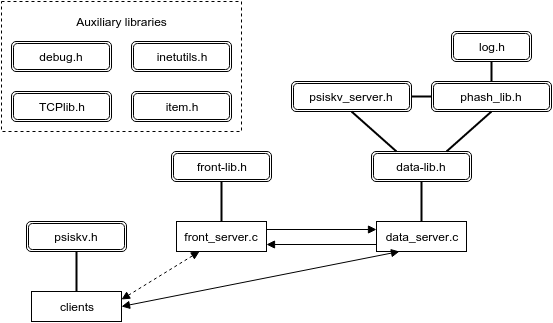
\includegraphics[width=0.8\textwidth]{./Pictures/KV_SystemOverview.png}
\caption{Overview of the system components and libraries}\label{fig:KVSyst}
\end{figure}

Figure \ref{fig:KVSyst} shows an overview of how the most important libraries and components of the system are connected.

\section{Key Value Data Structure}

The \textbf{data storage} is implemented on an \textbf{hash table} where each bucket of the
hash table is a \textbf{linked list} and each list entry holds the key and a pointer to the
value. See Figure~\ref{fig:DataOverview} for more details.

\begin{figure}[H]
\centering
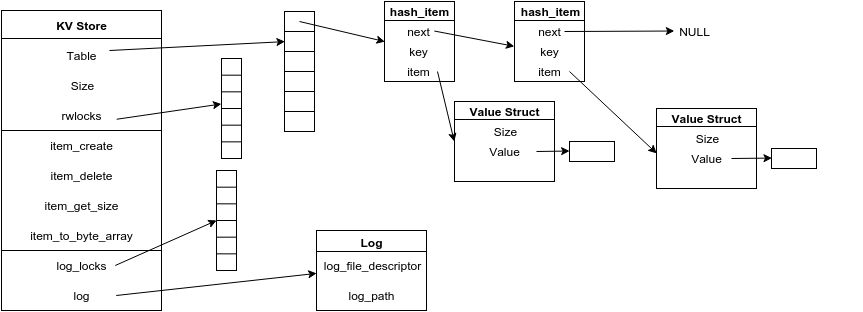
\includegraphics[width=\textwidth]{./Pictures/DataStructures.png}
\caption{Overview of Data Structures}\label{fig:DataOverview}
\end{figure}

The hash table component is implemented with \textbf{data abstraction} in mind,
in this system it holds a byte array and its size, but could be used to store any
kind of data. The item to be stored on the hash table is implemented in  another
component, in the key-value store case to the \emph{psiskv\_server.h}. There all necessary
auxiliary functions are implemented and a pointer to them is stored on the data structure.

\subsection{Backup and Log}
\label{sub:BackupLog}

To maintain data between data server executions a backup and a log file are used.
The backup stores a snapshot of the state of the Hash table, while the log stores
all successful write and delete commands made since startup.

At startup the data server initializes the hash table according to the flowchart
on figure~\ref{fig:BackupLogFlow}.

\begin{figure}[H]
\centering
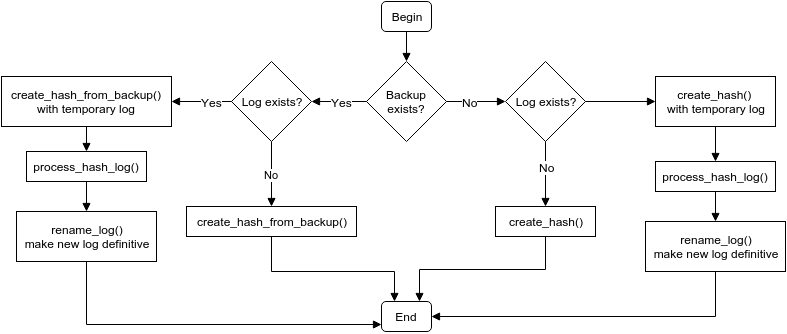
\includegraphics[width=\textwidth]{./Pictures/BackupLogFlow.png}
\caption{Data server hash table initialization flow}\label{fig:BackupLogFlow}
\end{figure}

At a clean exit the data server creates a new backup and deletes the log file.
Which means that there only exists a log file if the data server didn't exit orderly.

To prevent data consistency problems with faults during this process, the
backup file is only deleted after a new backup file is ready.

\subsection{Synchronization}
\label{sub:Synchronization}

As the Data Server is multi-threaded there might be problems with concurrent operations.
The hash table and the log file are vulnerable to these problems, so a mechanism was implemented to protect them.

There are three operations on the hash table susceptible to problems, \emph{read\_item}, \emph{insert\_item} and \emph{delete\_item}.
Has the hash table is divided into buckets the problematic situations occur with operations to items in the same bucket.
And so an array of readers-writer (RM) locks are stored in the hash table and lock access to each of the buckets.
Each of the buckets stores a linked list of hash\_items, so there are measures that need to be taken when cycling through the list.
For instance a while any operation searches for an item, no item deletion or insertion can occur on that list. So during the insert and delete operations the RW lock of that bucket is locked for writing and during a read is locked for reading.

The operations that are written to the log are the item insertion and deletion.
All write operations to the log are atomic, so there is no need to lock threads that aren't acting on the same bucket.
However, The system has to guarantee that operations to the same item are written in the order on which they are executed.
Because of this another array of mutexes controls the log operations.
These mutexes are locked right before the RW locks are unlocked on the insert and delete operation, to guarantee that the log is written right after the operation on the hash table.

\section{Key-Value Communication}

To use the Key-Value Store the client uses the \emph{psiskv.h} library to establish a
connection and make requests. The communication flow is exemplified on figure~\ref{fig:Comms}.
During the \textbf{kv\_connect} the \textbf{client} connects to the \textbf{Front Server} which responds
with the port of the \textbf{Data Server} and then the client connects to it and is ready
to make requests.

\begin{figure}[H]
\centering
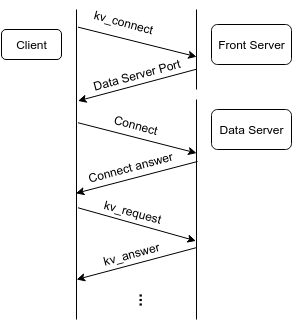
\includegraphics[width=0.6\textwidth]{./Pictures/CommunicationFlow.png}
\caption{Overview of the client KV store communication flow}\label{fig:Comms}
\end{figure}

The structure of the messages exchanged between the \textbf{client} and the \textbf{Data server}
is:  a  enumerate \emph{msg\_type}, a \emph{uint32\_t} with the \textbf{key} and an \emph{unsigned int}
with the length of the value. The possible message types are:
\begin{description}
    \item[WRITE\_REQ] - write request;
    \item[WRITE\_REQ\_OW] - write request with overwrite;
    \item[WRITE\_RESP] - write response;
    \item[READ\_REQ] - read request;
    \item[READ\_RESP] - read response;
    \item[DELETE\_REQ] - delete request;
    \item[DELETE\_RESP] - delete response;
    \item[ERROR] - error message;
\end{description}
After a \emph{WRITE\_REQ}, a \emph{WRITE\_REQ\_OW} or a \emph{READ\_RESP} a buffer containing
the value is transmitted over TCP with the length being specified on the previous
message.

%\subsection{Error Messages}
%\label{sub:ErrorMessages}
% TODO

\section{Inter Server Communication}
\label{sec:CommunicationProtocol}
To ensure that the processes keep each other alive, that the data server knows when
to shutdown and  that the front server knows the Data Server's address, the servers
have a communication protocol. One thread in each server, called 'communication
worker', exchanges the following messages:
  \begin{description}
    \item[PING] - default message, just to ensure the other process is still alive, 1 per second;
    \item['PORT'] - informs the Front Server about the Data Server's port;
    \item[EXIT] - commands the Data Server to shut down;
    \item[OK] - informs the Front Server that the Data Server received the EXIT command;
  \end{description}

The bilateral communication between servers is made using an Unix socket with
byte streams. To create this communication channel each server follows a small
algorithm. First they try to be the client, attempting to connect to the server.
If they succeed the system is ready. If that fails it means the other server isn't
running so they launch it, with a fork and a execv, and start accepting requests
on the unix socket. When they receive a connection the other server is ready. If
in the mean time the other server stops responding they re-launch it and wait for
it's connection.

\section{Front Server}
\label{sec:FrontServer}

The Front Server is a discovery server and a piece in the fault tolerance system for this project,
it serves to the clients as an interface to locate the data server, which is addressed at the lowest port he can
and communicates it to the front server using the communication system between them.

The Front Server also has a Command Thread to allow the apropriate shutdown of both the servers,
it works by listening to Stdin commands then, if and only if the command is "quit" it will send the command
to the Data Server and they'll both shutdown properly.

A flowchart of the execution of the Front Server is available on figure \ref{fig:CommunicationsFront}.
The communication to the data server and it's fault tolerance are also detailed.

\begin{figure}[ht]
\centering
\includegraphics[width=0.8\textwidth]{./Pictures/Communications-Front.png}
\caption{All communications with Front Server}\label{fig:CommunicationsFront}
\end{figure}

\section{Data Server}
\label{sec:DataServer}

The Data Server, which will be located at the first port it finds available,
works as a key-value store, that has four functionalities, such as read,
write, update and delete a value with a certain key. It is also a piece on the fault tolerance system,
by checking constantly if the Front Server is still alive and resurecting him if necessary.

The execution of the Data Server is depicted on the flowchart on figure \ref{fig:CommunicationsData}.

\begin{figure}[ht]
\centering
\includegraphics[width=0.9\textwidth]{./Pictures/Communications-Data.png}
\caption{All communications with Data Server}\label{fig:CommunicationsData}
\end{figure}

\subsection{Thread Management}
\label{sub:ThreadManagement}

The threads are created following the \textbf{on demand} strategy for both the front and
the data server.

On the front server there are three threads always running and others created
to handle kv\_connect requests. There is one thread reading from stdin to check if
the user tells the server to quit, there is the main thread, locked in a accept for the
TCP socket that creates new threads for each new request and the communication
socket, that exchanges messages with the data server, see section \ref{sec:CommunicationProtocol}.

On the data server there are two threads always running and others created
on demand to answer client requests. There is the main thread responsible for
creating threads to answer the clients and the communication thread.

\section{Fault Tolerance}
\label{sec:FaultTolerance}

Besides preventing data loss with the use of a backup and a log file, see section \ref{sub:BackupLog},
there are also mechanisms to recover from crashes on one of the the servers.
As specified, faults during recovery were ignored.

To detect a fault on one of the servers the communication protocol is used.
When one of the servers crashes, the conection between the communication
workers falls, at that point, the other server's connection worker will issue the pull
up command, it will fork the process, kill the binded servers in the new process and
call execv with the oposite server's filename, this one, when it's communication
worker is ready it connects to the other server's communication worker, in order
to reestablish the background connection and resume the fault tolerance.

%\section{Clients}
%\label{sec:Clients}
% TODO







\end{document}
